\documentclass[tikz]{standalone}
\usetikzlibrary{positioning,calc}
\begin{document}
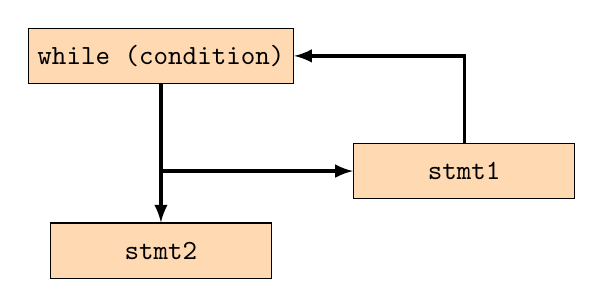
\begin{tikzpicture}[node distance = 9mm and 14mm,
  nodes= {draw, minimum width=8em, minimum height=2em, fill=orange!30,
    font=\ttfamily},
  arr/.style = {very thick,-latex}
  ]
  \node (while) {while (condition)};
  \node (stmt1) [below right=3.0em of while] {stmt1};
  \node (stmt2) [below=5.0em of while] {stmt2};

  \draw[arr] (while) |- (stmt1);
  \draw[arr] (stmt1) |- (while);
  \draw[arr] (while) -- (stmt2);
\end{tikzpicture}
\end{document}
